\section{Introduction}

The ``follow-the-renewables'' approach (the reader may consult Chapter 2 for more details) is an interesting strategy for mitigating the intermittency of renewable energy availability without the need to use energy storage devices. For example, when it is night in the location where a DC A resides, the workload could be migrated to another DC B where the sun is still shining to use solar power---as seen in Figure~\ref{fig:ex_follow_the_renewables}.

Despite its benefits, one cannot neglect the limitations of the follow-the-renewables strategy. First, the process of migrating a VM between different DCs consumes energy itself: it uses network devices (such as switches and routers) and a computational task for the live migration process. The scheduling algorithm must consider this energy consumption before deciding if the migration is advantageous. Second, the network communications links that connect the servers inside the DC and the different DCs can suffer from congestion, which may increase migration duration. This results in unnecessary computation and energy consumption on both the origin and the target servers: the server that is sending the VM needs to wait for the migration process to finish to free its resources and receive additional VMs, or it could be turned off as well to save energy; the server that is receiving the VM will only start executing the new VM after the end of the migration process. An efficient scheduling algorithm must consider those factors to decrease the carbon footprint of the DCs operations.


The work by Camus et al.~\citet{SAGITTA,NEMESIS} studied the scheduling of the cloud workload, in the form of virtual machines (VMs), on geographically distributed DCs to minimize non-renewable energy consumption. It proposed different stochastic models to estimate renewable energy production and greedy heuristic algorithms to allocate tasks to servers. VMs are allowed to be migrated during execution to a computer within the same DC (intra-DC server consolidation)  or to a computer in a DC located in another geographic location (``follow-the-renewables''). The scheduling algorithm considers the network cost of the migration.


This chapter presents an extension of this work with an analysis of the indirect impact of using the follow-the-renewables approach in energy consumption. This impact can be divided into two categories: direct and indirect. The network devices' energy consumption causes the direct impact, and since the power consumption does not vary significantly based on the device usage~\cite{energy_network_devices}, we assume the network devices' power consumption to be static. For the indirect impact, it is generated by the live migration of the VMs, which uses the network to transfer all the data related to the task to the destination machine, as well as the computational task required to perform this live migration. More specifically, this chapter presents the following contributions:


\begin{itemize}
    \item an analysis of the impact of not considering the network (bandwidth, latency, and topology) in both energy consumption and network congestion;
    \item an accurate estimation algorithm for the time it takes to migrate a virtual machine that takes into account the network topology, link bandwidth, and latency;
    \item a scheduling algorithm for the live migration of the VMs that uses the estimation algorithm and has the same or lower brown energy; consumption than the baselines, with no network congestion.
\end{itemize}
    
The work of this chapter resulted in the following publication:  \textit{\textbf{Miguel Felipe Silva Vasconcelos}, Daniel Cordeiro and Fanny. ``Indirect network impact on the energy consumption in multi-clouds for follow-the-renewables approaches''. In Proceedings of the 11th International Conference on Smart Cities and Green ICT Systems — SMARTGREENS 2022, pages 44–55. INSTICC, SciTePress}. The text of the present chapter is an adaptation of this publication.

This chapter is organized as follows. In Section~\ref{sec:nemesis}, the model of~\citet{NEMESIS}, the foundation of this work, is summarized. Section~\ref{sec:modeling_smargreens} details the new scheduling method for the migrations, while Section~\ref{sec:simulations_smargreens} is devoted to simulations parameters. Results are detailed in Section~\ref{sec:results_smargreens}. Finally, Section~\ref{sec:conclusion_smargreens} summarizes the chapter.


\section{The NEMESIS algorithm}
\label{sec:nemesis}

In this section, we describe the resource management framework NEMESIS~\cite{NEMESIS}, which was the foundation for the work presented in this chapter. The NEMESIS algorithm manages a multi-cloud composed of DCs geographically distributed across a country. The DCs power demand is supplied from the regular electrical grid and locally installed PVs. Given the intermittency of renewable energy, the NEMESIS algorithm uses the stochastic modeling of SAGITTA~\cite{SAGITTA} to obtain the expected value of the renewable energy available at a given time to be used as input for the scheduling algorithms.

NEMESIS has a central controller, and the workload execution is scheduled in 5-minute time slots. The workload consists of heterogeneous VMs in terms of the number of CPU cores, RAM size, and requested execution time. The scheduling decision uses greedy heuristics inspired by the Best-Fit algorithm. While it may not result in the optimal solution, greedy heuristics can provide an acceptable result in a reasonable amount of time, and these characteristics are relevant for the scenario of cloud computing, where millions of VMs are submitted per hour and a significant portion of these tasks have strict quality of service requirements and cannot be delayed. The scheduling algorithm has four main steps, detailed as follows.

In the first step of the algorithm (pre-allocation of the incoming VMs), the controller will search for servers to allocate the VMS received during the time slot. There are two restrictions for this scheduling algorithm: i) the server has available computational resources to host the VM;  and ii) executing the VM in this server would result in the minimum increase in the expected brown energy consumption. The algorithm first sorts the VMs by their volume (a product of the number of CPU cores and the amount of RAM) in decreasing order and then performs the search for each of the VMs. If a server is found that respects the two restrictions, the algorithm makes a reservation (pre-allocation) for the VM being analyzed and goes to the next VM. On the other hand, if no server is found, the VM will be delayed to be processed in the next time slot.

The second step of the algorithm (revision of the pre-allocations) performs a revision of the reservations made by the previous step, given that the greedy heuristic used may not provide the optimal solution.  The strategy is to move the reservation from the DCs expected to consume more brown energy to the DCs expected to have the most availability of green energy.  There are two constraints for this algorithm: i) there exists a server in the DC being evaluated that can host the VM; and ii) the expected brown energy is reduced.

The availability of green energy may change during the execution of the VMs, and the third step of the algorithm (migration of the running VMs) aims to reduce brown energy consumption by migrating the running VMs. It uses the same strategy as the second step of the algorithm (moves the workload from DCs using more brown power to DCs that have more green power available) and with the following restrictions: i) the migration needs to finish before the beginning of the next time slot; ii) the remaining execution time of the VM needs to be greater than the duration of the migration process; iii) one DC can only migrate to another 2 DCs during a time slot; and iv) the migrations from one DC are planned to execute one after another, that is, they cannot happen simultaneously in parallel. Restrictions (iii) and (iv) are simple heuristics to avoid network congestion with the load generated by the VM live migrations.

The power demand from the servers accounts for approximately half of a data center's overall energy consumption~\cite{power_to_the_people}. The last step of the algorithm (server consolidation) aims to minimize the number of active servers. In this process, the algorithm assesses if it can redistribute the running VMs (by executing live migrations within the data center, referred to as intra-DC migrations) to decrease the number of servers in use and shut down the servers that become idle.

\subsection{Cloud Modeling}\label{sec:cloud_model}

NEMESIS cloud modeling is based on a real cloud infrastructure: the Grid'5000 testbed\footnote{Grid'5000 testbed: \url{https://www.grid5000.fr}. Accessed on October 20, 2023.}. It is considered a subset of the original platform with 1035 servers distributed among 9 data centers in France and Luxembourg: 116 servers in Grenoble; 74 servers in Lille; 38 servers in Luxembourg; 103 servers in Lyon; 240 servers in Nancy; 44 servers in Reims;  129 servers in Rennes;  151 servers in Sophia Antipolis; and 140 servers in Toulouse. The servers are considered homogeneous in terms of memory, CPU, and energy consumption, and are based in the Taurus node of the Grid'5000, equipped with two Intel Xeon E5-2630 CPUs (6 cores per processor), and 32 GB RAM.

The network is modeled both for the connection of the servers inside the DCs (network links with 1 Gbps of bandwidth) and the connection between the different DCs  (network links with 10 Gbps bandwidth). Figure~\ref{fig:topology} depicts the cloud platform's network topology (the DCs' placement was not based on their geographic location, but to visualize the network links better). One can observe that multiple DCs share some network links, thus the migration planning needs to consider this information to avoid generating network congestion and the resulting waste of resources.

\begin{figure}[h]
  \centering
   {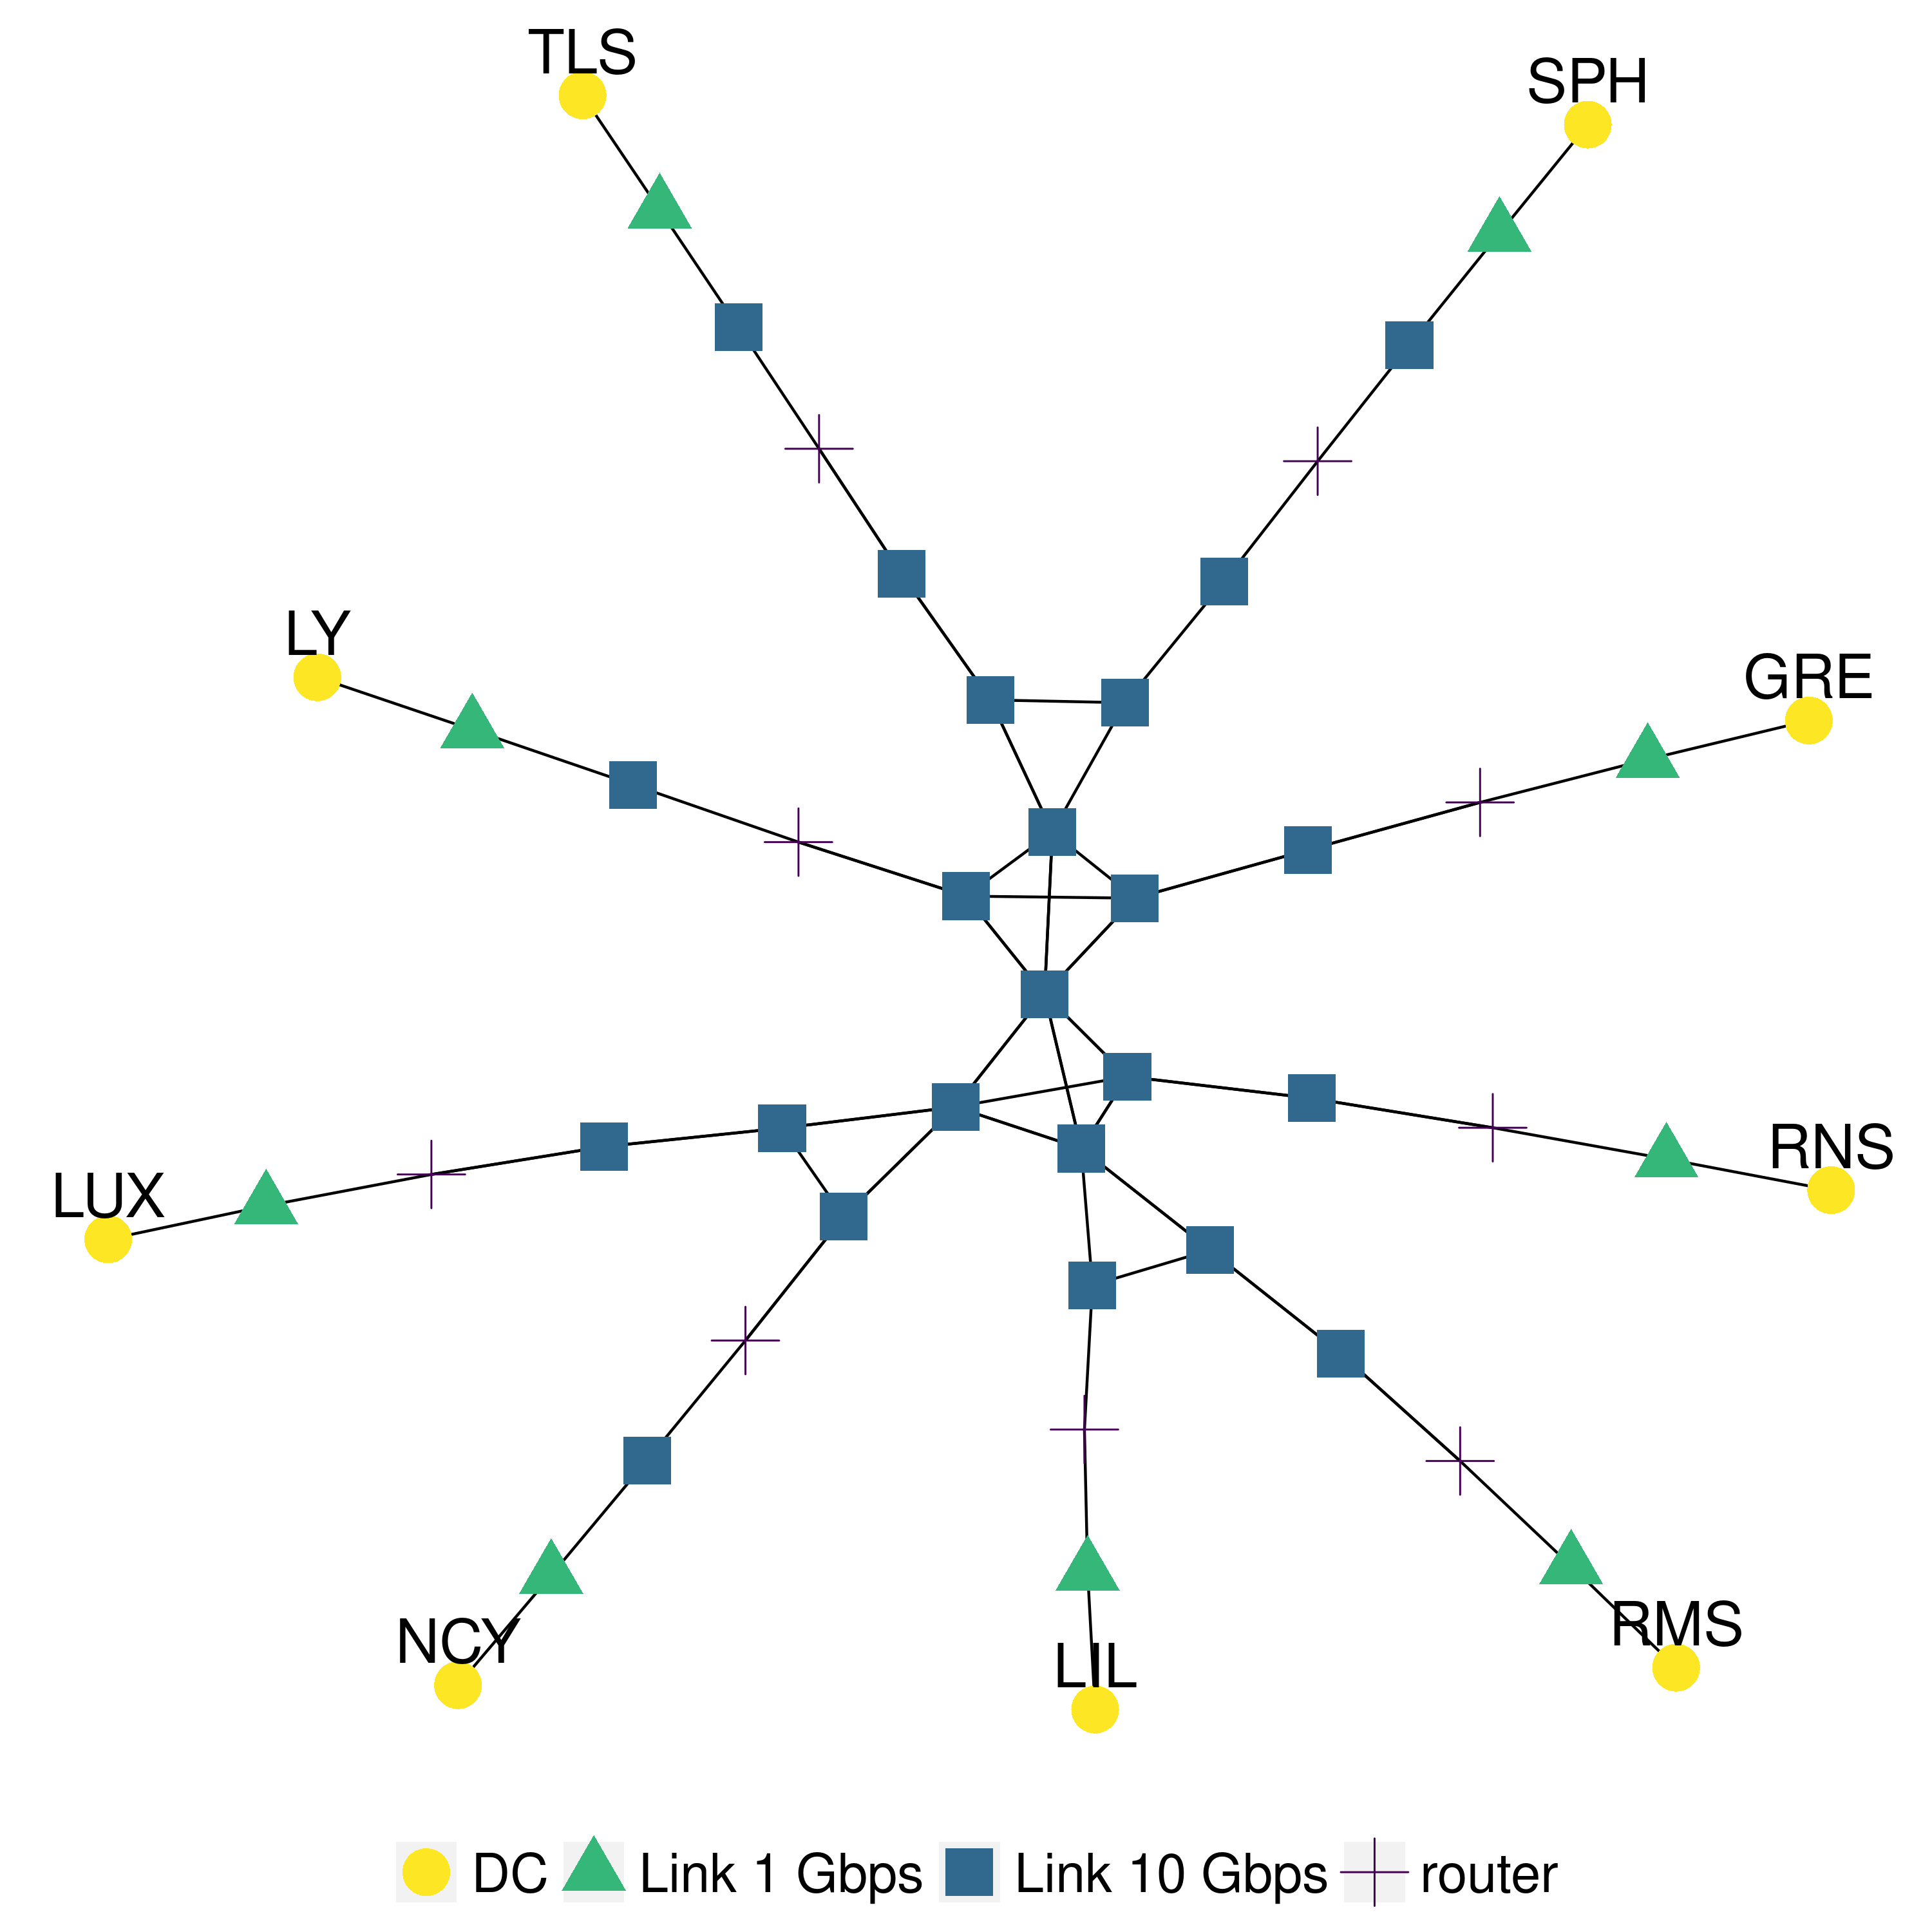
\epsfig{file = images/topology.PNG, width = .7\textwidth}}
  \caption{Topology of the Cloud platform, where ``GRE'' is Grenoble,  ``LIL'' is Lille, ``LUX'' is Luxembourg,``LY'' is Lyon, ``NCY'' is Nancy, ``RMS'' is Reims,  ``RNS'' is Rennes, ``SPH'' is Sophia, and  ``TLS'' is Toulouse.}
  \label{fig:topology}
 \end{figure}
 

Regarding the energy consumption of the servers, it is considered a linear model based on CPU usage, and the VMs always use 100\% of the requested number of CPU cores. The server presents a fixed consumption for its IDLE state (97~W), and the power consumption based on core usage is as follows: 128~W for 1 core; 146.4~W for 2 cores; 164.8~W for 3 cores; 183.2~W for 4 cores; 201.6~W for 5 cores; and 220~W with 6 cores. Furthermore, the energy consumption of turning on a server (127~W during 150 s), turning off a server (200 W for 10 s), and when the server is off (8 W) are modeled as well. 


\subsection{VM live migration model}

The VM live migration model of NEMESIS has three phases. In the first phase, all the memory pages of the VM are transferred to the destination server. In the second, after completing the copy of all the memory pages, a message is sent to notify the end of the stop-and-copy step. Finally, in the last step, the commitment message is sent to the new host to inform them of the end of the migration process, and the VM will be destroyed on the server of origin and resumed on the destination host.


\section{The c-NEMESIS algorithm}
\label{sec:modeling_smargreens}

In this section, we present how we extended the NEMESIS algorithm to perform the analysis of the impact of the follow-the-renewables in both network and energy. The new algorithm is called c-NEMESIS, where the ``c'' stands for congestion and its full name is ``Congestion and Network-aware Energy-efficient Management framework for distributEd cloudS Infrastructures with on-Site photovoltaic production''. Section~\ref{sec:estimating_mig_duration} presents how the algorithm for estimating the duration of the migration process was updated, and  Section~\ref{sec:planning_migrations} shows the modification in the migration scheduling algorithm. Finally, Section~\ref{sec:energy_costs_mig} presents how we model the energy consumption of the live migration process.


\subsection{Estimating the duration of the live migration}
\label{sec:estimating_mig_duration}

The duration of the migration is essential information for the scheduling decision, as it can help avoid oversaturating the network links and generating network congestion. Algorithm~\ref{alg:estimation} is an extension of the NEMESIS algorithm, and it executes this estimation, where: \textit{linkLatency} is the latency of the link; \textit{routeSize} is the number of links that interconnects the host where the VM is originally running to the target host of the migration; \mbox{\textit{windowSize}} = 4,194,304 Bytes, is the TCP maximum window size; \textit{bandWidthRatio} = 0.97, represents the additional load caused by the headers of TCP/IP; \textit{bandwidth} = the minimum bandwidth among the links that interconnect the host of origin with the target host; $\alpha$ = 13.01, simulates the TCP slow start factor, that is, not all the bandwidth is instantly available for the communication; and $\gamma$ is used to represent the Bottleneck effect of the TCP protocol. The parameters used in Algorithm~\ref{alg:estimation} were based on the study from~\citet{velho2013simgridparameters}. 

The difference between Algorithm~\ref{alg:estimation}  and NEMESIS is the \textit{routeSize} variable: NEMESIS used fixed values (5 for live migrations intra-DC, and 11 for live migrations inter-DC), and now it is assumed that the cloud operator has information about the network topology of his DCs, thus the real number of links that interconnect the two hosts is used.

\begin{algorithm}[h]
\begin{algorithmic}
\caption{Estimation of the migration duration.}\label{alg:estimation}
\State $theLatency \gets linkLatency \cdot routeSize$
\State $transferLat \gets theLatency + \frac{\gamma}{bandwidth}$
\State $throughputL \gets \frac{windowSize}{2 \cdot transferLatency}$
\State $throughputB \gets bandwidth$
\State $throughput \gets min(throughputL, throughputB)$
\State $throughput \gets throughput 
\cdot bandWidthRatio$
\State $timeToMigrate \gets  3 \cdot \alpha \cdot transferLat + \frac{vmRamSize}{throughput}$ 
\end{algorithmic}
\end{algorithm}

\subsection{Planning the migrations}
\label{sec:planning_migrations}


Algorithms~\ref{alg:general} and~\ref{alg:detailed} plan the VM migrations considering the network topology and the bandwidth usage. They are inspired in the migration planning of NEMESIS, with the following modifications: i) the available bandwidth of the links is considered (it changes based on the number of migrations that use the same network link); ii) migrations can be performed in parallel between different DCs respecting the links' bandwidth constraint; iii) the intra-DC migrations (for the server consolidation) are sequentially distributed in time (do not execute simultaneously) ; iv) the real number of links that interconnect the origin and the target server is used as input for the estimation algorithm of the migration duration.

\begin{algorithm}[h]
\begin{algorithmic}
\caption{Migration planning at mulit-cloud level.}\label{alg:general}

\State $DCs$ \Comment{Sorted by increasing ERGE}
\State $plannedTime \gets 0$
\State $timeSlotDuration \gets 300$
\State $linksHistory \gets \emptyset$
\While {$plannedTime < timeSlotDuration$}
\State $dc\_tx \gets $ first item of $DCs$  %\Comment{DC where the VM is initially running}
    \While {$dc\_tx \neq$ last item of $DCs$}
        \State $dc\_rx \gets $ last item of $DCs$
        \If{$dc\_tx$ has VMs that can be migrated}
            \While{$dc\_tx \neq dc\_rx$}
            \State plan migrations between $dc\_tx$ and $dc\_rx$ using Alg.~\ref{alg:detailed}
            \State $dc\_rx \gets$ previous DC of $DCs$
            \EndWhile
        \EndIf
        \State $dc\_tx \gets$ next DC of $DCs$
    \EndWhile
    \If{no VM migration was planed and no migration is in execution }
       \State \textbf{exit}
    \EndIf
    \State $plannedTime \gets$  instant after the expected end of next migration 
\EndWhile
\end{algorithmic}
\end{algorithm}


\begin{algorithm}[h]
\begin{algorithmic}
\caption{Migration planning between two DCs.}\label{alg:detailed}
\Require $dc\_tx,dc\_rx$

\State $VMs \gets$ list of VMs of $dc\_tx$
\For{$vm$ in $VMs$}
    \State $origin \gets$ server where the $vm$ is running
    \State $target \gets$ server from $dc\_rx$ being evaluated
    \State $worth \gets brownMig < brownNotMig $
    \State $e\_time \gets $ estimate the migration time using Alg.~\ref{alg:estimation} 
    \State $band\_ok \gets$ links between $source$ and $target$ can receive the additional load of the migration
    \If{ $worth$ and $band\_ok$ }
    \State registers the planning of the migration and updates the link history   
    \EndIf
\EndFor

\end{algorithmic}
\end{algorithm}

Algorithm~\ref{alg:general} is used to plan the migrations of the multi-cloud. Initially, the DCs are sorted by increasing order of expected remaining green energy (ERGE). Let $dc\_tx$  be the index of the position of the DC with the least available energy---initially at the beginning of the list, and it will be the candidate to send VMS, and $dc\_rx$ the index of the position of the DC with the most green energy---initially at the end of the list, and it is the candidate to receive the VMs. The main idea of the algorithms is to migrate VMs from the DCs that are expected to use brown energy to the DCs that are expected to have green energy. 

In order to evaluate if it is possible to migrate VMs from $dc\_tx$ to $dc\_rx$ and if it is worth---the brown energy consumption will be reduced---Algorithm~\ref{alg:general} uses the Algorithm~\ref{alg:detailed}, which works as follows. 
First, the algorithm extracts the information about the running VMs (grouped by the servers) of the DC $dc\_tx$. The planning starts at the beginning of the time slot. For each VM that can be migrated, the algorithm tries to find a server in the destination DC $dc\_rx$ with the following restrictions: i) it has available computational resources to host the VM (CPU and memory); ii) the links that interconnect the server of origin (where the VM is running) and the target server can receive the additional load of the migration without violating their bandwidth constraint; iii) the VM migration finishes during the current time slot (if the destination server is off, the time to turn the server on is taken into account); and iv) performing the migration reduces the expected brown energy consumption. 

If all these restrictions are respected, the VM is planned to migrate, and the algorithm registers in the \textit{linkHistory} that the links that connect these two servers will be used until the instant when the VM migration is expected to finish in order to compute the available bandwidth of the network links.  If there are still remaining VMs that could be migrated from DC $dc\_tx$, the algorithm will try to migrate them to DC $dc\_rx -1 $, and so on, until all the VMs from DC $dc\_tx$ are planned to be migrated or all the DCs are processed. After finishing processing the DC $dc\_tx$, the algorithm repeats the same process for the DC $dc\_tx +1$ until all the DCs are processed.

After evaluating all the possible migrations for the instant at the beginning of the time slot, the algorithm will use the link usage history to obtain information about when there will be available links in terms of bandwidth---at what instant of time \texttt{t} the next migration is expected to finish.  If there are still VMs that could be migrated, the migration planning algorithm will be executed again using the availability of the bandwidth at the instant \textit{t}. Then, the process repeats until there are no more VMs to migrate, or the evaluation time reaches the end of the time slot.

Regarding the server consolidation, there are two differences to the original NEMESIS algorithm: i) it will only be applied to the DCs that didn't have inter-DC migrations planned to avoid generating network congestion---given that the intra-DC migrations could use the same network links as the inter-DC migrations planned in the previous step; and ii) the migrations are distributed in time using the estimation computed with Algorithm~\ref{alg:estimation} to avoid overlapping them.


The computational complexity of the Algorithm~\ref{alg:detailed} is $O(n_{VMS} \times  n_{servers} \times n_{links}  )$, where $n_{VMS}$ is the number of running VMs on the DC that is sending the VM, $n_{servers}$ is the number of candidate servers that have the least possible amount of free cores to run the VM on the destination host, and $n_{links}$ represents the number of links that interconnect the VM's host of origin and the target host. For Algorithm~\ref{alg:general}, the computational complexity is given by $O(n_{DCs}\log{}n_{DCs} + {n_{DCs}}^{2} \times n_{VMS} \times  n_{servers} \times n_{links})$, where $n_{DCs}$ is the number of DCs.

\subsection{Energy cost of migrations}\label{sec:energy_costs_mig}

The energy consumption of a live VM migration is modeled in NEMESIS by a computation task executed on the target host. This task uses 100\% of a single CPU core during the migration process. Suppose the migration is impacted by network congestion. In that case, its duration will increase, resulting in a waste of energy on the server where the VM was initially running as well as on the target server.


The wasted energy is proportional to the extra time migrating, that is, the difference between the duration of the migration process compared to the duration that it would take if there were no network congestion. A lower bound for the wasted energy can be computed with Algorithm~\ref{alg:wasted_energy} using as input this extra time migrating. Given that the migration planning uses a ``follow-the-renewables'' approach to move the workload from the DCs that are using brown power at that instant to the DCs that have more available green energy, the algorithm computes individually the wasted energy in the server that is sending the VM and in the server that is receiving the VM. For the server that is sending the VM, this extra energy consumed is brown(er), increasing the overall brown energy consumption of the cloud, since this server could be turned off to save energy. For the server that will receive the VM, this extra energy is green(er), but it is wasted because it was only available at that instant (no energy storage devices) and could have been used to execute the workload.

\begin{algorithm}[h]
\begin{algorithmic}
\caption{Extra energy consumption of migrating.}\label{alg:wasted_energy}

\State $pCore \gets 20.5$

\State $wastedOrigin \gets 0$
\State $wastedTarget \gets 0$

\For{$mig$ in $Migrations$}
    \State $vmCores \gets$ amount of cores of the VM being migrated
    \State $extraTime \gets mig.Time - mig.TimeNoCong$
    \If{$extraTime > 0$}
        \State $wastedOrigin += extraTime \cdot pCore \cdot vmCores$ 
        \State $wastedTarget += extraTime \cdot pCore$ 
    \EndIf
\EndFor
\end{algorithmic}
\end{algorithm}

The value of \textit{pCore} is an estimate for the additional cost of executing a core, and is obtained as follows: the server consumes \SI{220}{\watt} at full load and subtracting the power consumption of the IDLE state (\SI{97}{\watt}) it results in \SI{123}{\watt}. Finally, this value is divided by the total number of cores on the server (6), resulting in \SI{20.5}{\watt}. Notice that \textit{pCore} is only multiplied by the number of cores of the VM for the server of origin, since it remains executing in the VM until the end of the migration, and on the destination server the computational task uses only a single CPU core.

\section{Experiments}

\label{sec:simulations_smargreens}

In this section, we describe the experiments performed to evaluate the impact of the follow-the-renewables approaches in both energy and network, considering one week of operating the multi-cloud. Section~\ref{sec:settings_smartgreens} presents the settings used to execute the experiments. To further evaluate the effectiveness of using ``follow-the-renewables'' approaches, we detail in Section~\ref{sec:baselines_smartgreens} two other works that incorporate this approach in different ways and are used as baselines for the c-NEMESIS algorithm. Finally, Section~\ref{sec:results_smargreens} discusses the obtained results. 
 
 The results of the experiments are deterministic. Therefore, only results for a single execution of the simulations are presented. A public Git repository hosts all the simulation code, inputs, and the instructions to run and extract the results\footnote{Git repository with the c-NEMESIS reproducible artifact: \url{https://gitlab.com/migvasc/c-nemesis}. Accessed on October 20, 2023.}. 


The experiments were performed using computational simulations. The Simgrid~\cite{CASANOVA20142899} framework (version 3.28) was used to develop the simulations because it allows modeling distributed computing experiments, such as cloud platforms, in particular: energy consumption of executing the tasks, turning on and off the servers, network usage by the live migration process, network topology and network congestion. Another relevant reason for choosing the Simgrid framework is the fact that it is well-validated by the scientific community, with over 20 years of usage. For the network, the default flow-level TCP modeling of Simgrid produces precise results for large distributed computing scenarios (as in our case with thousands of servers) in a reasonable amount of time. It is possible to use packet-level simulation, however, despite being more precise, it would result in a huge execution time for the simulations~\cite{velho2013simgridparameters}. 


\subsection{Settings}

\label{sec:settings_smartgreens}

The cloud infrastructure is based on the adapted version of Grid'5000 (same as NEMESIS, see Section~\ref{sec:cloud_model}) for the network topology,  server hardware specifications and power consumption.

\subsubsection{Workload}

Traces from real cloud providers were used to generate the workload for the experiments. The data extracted from the traces were the number of CPU cores requested, the instant of time when the task was submitted, and its duration. Regarding the requested RAM per VM, it is considered that each VM will consume 2 GB per core requested, similar to the \texttt{t2.small} instance of Amazon EC2\footnote{Amazon EC2 instance types: \url{https://aws.amazon.com/ec2/instance-types/}. Accessed on October 20, 2023.}. It is also considered that the VMs execute with full CPU usage of the requested cores, the worst scenario for energy consumption. 

The workloads are scaled to use a maximum of 80\% of the computational resources of the cloud platform at any given simulated time. This decision ensures that the tasks will always be allocated to the servers, and that there will be some room for the servers to receive VMs from live migrations, thus allowing for the analysis of the different scheduling approaches. Furthermore, from the cloud traces, it is possible to observe that the DCs are not used 100\% of their computational capacity. Figure~\ref{fig:workload} illustrates the number of VMs submitted during the week (in yellow), and the cumulative demand of CPU cores requested at a given time (in purple)---the total number of CPU cores used by the VMs in execution at that instant of time.

\begin{figure}[h]
  \centering
   {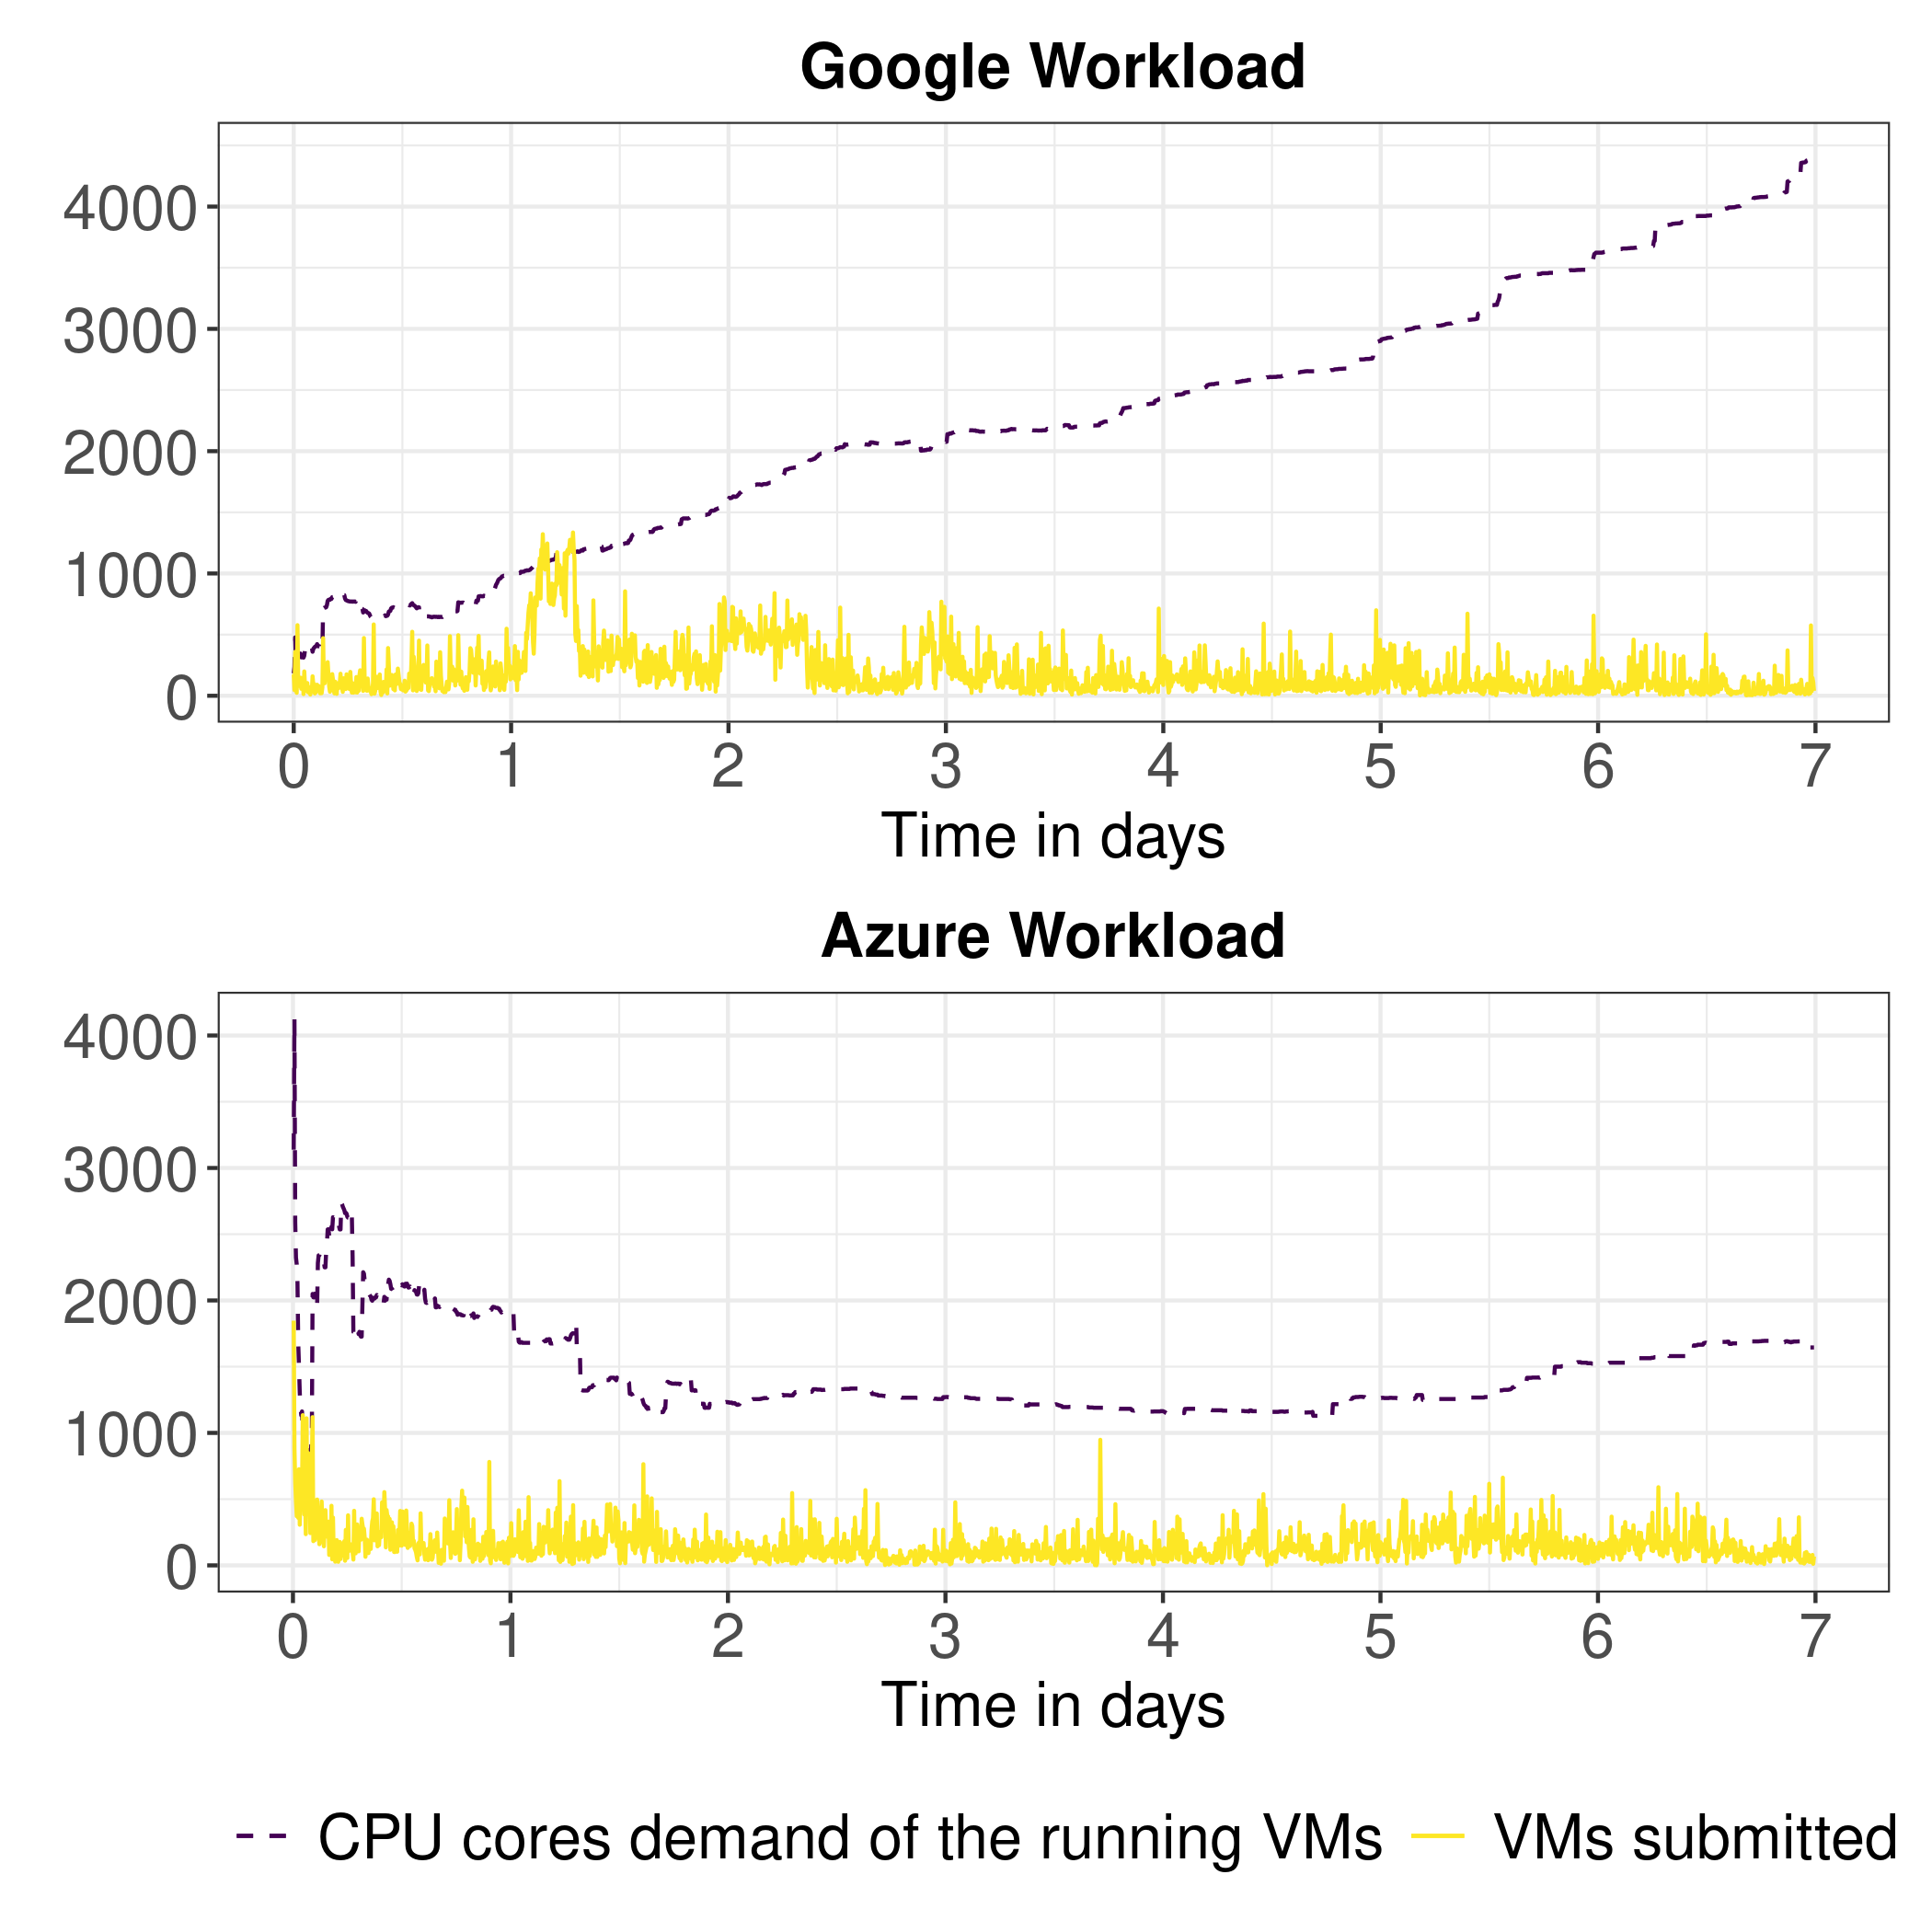
\epsfig{file = images/workloads.png, width = .9\textwidth}}
  \caption{Workloads used as input for our simulations.}
  \label{fig:workload}
 \end{figure}

The first workload was generated using as a base the 2011 Google Cluster Workload traces~\cite{google2011traces}, and it consists of over 380,000 VMs. In this workload, the VMs have a long execution time, as can be seen in Figure~\ref{fig:workload}, in which the value of the running VMs' CPU core demand keeps increasing throughout the week. The second workload was based on traces from Microsoft Azure~\cite{hadary2020protean}, more specifically, the Azure Trace for Packing 2020, and contains over 304,000 VMs. This generated workload has a different behavior than the previous one: there is a peak in the VM submissions at the beginning of the week, and the VMs have a shorter execution time, as seen by the fact that the CPU core demand does not keep increasing during the week.

These traces do not provide data about the network usage of the tasks, which was not modeled in the simulations. The additional load on the network is generated only by the live migration of the VMs. Therefore, this work can be seen as a lower bound for the real-world scenario.


\subsubsection{Green energy traces}

The data for the energy produced by the solar panels were obtained from the Photovolta\footnote{Photovolta project: \url{http://photovolta.univ-nantes.fr/}. Accessed on October 20, 2023.} project by \textit{Université de Nantes}. The data represents the power production of two arrays of 4 PVs each (Sanio HIP-240-HDE4) with a total nominal power production of 1920 Wc at intervals of 5 minutes. In order to simulate the different productions of the geographically distributed DCs,  a different week of the production trace was used for each DC. Furthermore, each DC had three PV panels per server. The PVs installed in the DCs generated the following amount of energy during the simulated week: i) Grenoble: 1.58 MWh; ii) Lille: 0.07 MWh; iii) Luxembourg: 0.15 MWh; iv) Lyon: 1.19 MWh; v) Nancy: 2.16 MWh; vi) Reims: 0.38 MWh; vii) Rennes: 1.63 MWh; viii) Sophia: 1.75 MWh; and ix) Toulouse: 1.53 MWh. In total, around 10.5 MWh of green power was produced in the simulated week. Figure~\ref{fig:green_power} shows the green power production per DC during the simulated week.

 \begin{figure}[h]
  \centering
   {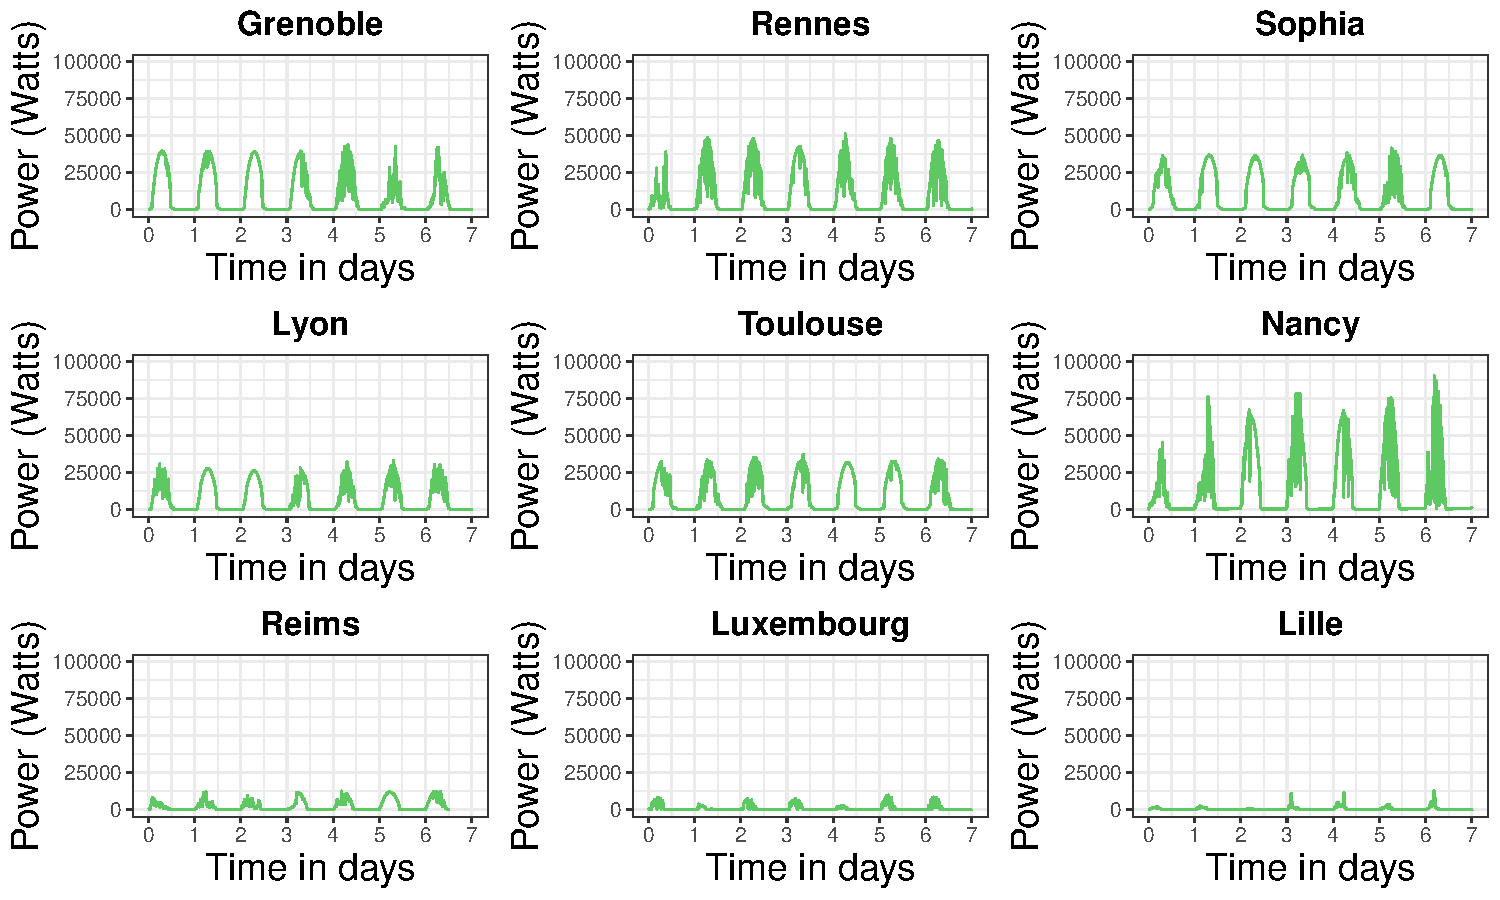
\epsfig{file = images/pv_pow_photovolta.pdf, width = \textwidth}}
  \caption{Green power production (in Watts) produced by DC during the
  simulated week.}
  \label{fig:green_power}
\end{figure}


\subsection{Baselines}
\label{sec:baselines_smartgreens}

The first baseline is the Workload shifting non brownout (WSNB) algorithm~\cite{XU2020191}. The algorithm works as follows. Initially, the VM is allocated to the nearest DC (aiming to reduce the response time) and to the server that will increase the energy consumption by the least (a server that is already on and its available computational resources are equal to or slightly greater than the requirements of the requested VM). Then, suppose this initial DC does not have available renewable power to execute the VM. In that case, the algorithm will evaluate another DC (the DCs are sorted by available green energy) that matches this demand and does not exceed a threshold for the response time. If another DC is found, the VM will be reallocated to it. The algorithm does not perform server consolidation with live migrations, it tries to use the minimum number of servers during this allocation. To adapt this baseline for the experiments, the response time restriction was removed from the algorithm, that is, we consider that all the DCs are homogeneous in terms of latency for the VM request, since the used workloads do not have this data, and this modification does not change the behavior of the algorithm.


The second work used as a baseline is the FollowMe@Source (or FollowMe@S) algorithm~\cite{ALI2021110907} that has two variants: i) FollowMe@S Intra, which only performs VM migrations inside the same DC (intra-DC migrations);  and ii) FollowMe@S Inter, that only performs VM migrations between different DCs (inter-DC migrations). Both algorithms have the same general steps, described as follows.

The FollowMe@S algorithm has two main steps: allocation and migrations. The allocation step begins by sorting the DCs by the availability of green energy. Then, the algorithm will search for a server that can host the VM, respecting the sorted list of DCs. If no server is found after searching through all DCs, the VM will be processed in the next scheduling round. The process will be executed again for all the other VMs to be scheduled. 

In the migration step, either exclusively intra-DC or inter-DC migrations are performed. First, the algorithm obtains a list of all the VMs that are in execution at that instant of time. Then, it evaluates the usage of the servers to identify the underutilized hosts (less than 20\% of CPU usage) and marks them to be turned off. The running VMs of these underutilized hosts will be removed using live migrations in order to turn them off and save energy. In the intra-DC case (FollowMe@S Intra), the algorithm will run in each DC separately. For each VM, it will try to find a server with available computational resources to host it, and the migration is performed if a server is found. In the inter-DC case (FollowMe@S Inter), for each VM that can be migrated, the algorithm will evaluate the DCs sorted by the availability of green energy, and migrate the VM to the server of the first DC that can host the VM. One important point to notice is that FollowMe@S does not consider the network when scheduling its migrations. The following modifications were performed to the algorithm to adapt it for the experiments: i) it is not considered the network costs of a distributed algorithm, since NEMESIS, c-NEMESIS, and WSNB are centralized algorithms; ii) the workload degradation of performance by migrating the VM---for example, migrating to a server with a less efficient CPU---is not modeled as a homogeneous platform is used.

The baselines adopt the ``follow-the-renewables'' approaches in different ways. The algorithms WSNB and FollowMe@S Intra only use ``follow-the-renewables'' for the initial scheduling, and the VMs are not migrated to other DCs during their execution. On the other hand, the algorithm FollowMe@S Inter performs VM migrations to other DCs---the same strategy adopted by NEMESIS and c-NEMESIS.



\subsection{Results}

\label{sec:results_smargreens}

In this section, we present the results of the simulations. First, Section~\ref{sec:accuracy_smartgreens} shows an analysis of the accuracy of an essential component of NEMESIS and c-NEMESIS algorithms: the algorithm for the duration of migration (Algorithm~\ref{alg:estimation}). Then, Section~\ref{sec:analysis_vms_migs_smargreens} provides an overview of the live migrations performed. Results from the energy consumption---total and brown---of the multi-cloud platform are shown in Section~\ref{sec:energy_smartgreens}. Finally, Section~\ref{sec:wasted_resources_smartgreens} discusses the impact of live migrations on network congestion and waste of energy.

 \subsubsection{Accuracy of the estimation algorithm}
 \label{sec:accuracy_smartgreens}
 We define an \emph{underestimated migration} as a VM live migration process with a longer duration than estimated. Table~\ref{tab:migs_under} presents the number of live migrations that were underestimated by NEMESIS and c-NEMESIS, and the percentage value that is based on the total number of migrations (that can be found in Table~\ref{tab:amount_migs}). For both workloads, c-NEMESIS presented almost no underestimation for the migrations compared to NEMESIS. Furthermore, it is interesting to notice that virtually all the intra-DC migrations were underestimated in NEMESIS because they started simultaneously, resulting in network congestion.
 
\begin{table}[h]
\caption{Number of underestimated live migrations and the ratio of the overestimation, where ``W'' stands for ``Workload'', ``G'' for Google, and ``A'' for Azure.}\label{tab:migs_under} \centering
\begin{tabular}{|l|c|r|r|}
  \hline
  \textbf{Algorithm} & \textbf{W}  & \textbf{Inter} & \textbf{Intra}   \\
  \hline
  NEMESIS  & G & 245 (4.4\%)   & 3 393 (95.7\%) \\
  \hline
  c-NEMESIS & G & 0 (0\%)  & 61 (2.9\%) \\
  \hline
  NEMESIS & A & 140 (3.6\%)   &  3 324 (94.1\%)   \\
  \hline
  c-NEMESIS & A & 24 (0.1\%)   & 49 (3.8\%) \\
  \hline  
\end{tabular}
\end{table}


In order to evaluate the estimation algorithm for the duration of the migrations, two metrics are used to assess its accuracy: the Mean Absolute Percentage Error (M.A.P.E.) and the Root Mean Square Error (R.M.S.E.). The M.A.P.E. is defined by: $ \frac{1}{n}\sum_{i=1}^{n}  \frac{| R_{i} - F_{i}|}{R_{i}}$, where $n$ represents the amount of values being considered, $i$ the index of the value being considered, $R_{i}$ the real duration of migration, and $F_{i}$ the estimated duration. The result of the M.A.P.E. is a percentage value, and it represents the relative value of the estimation errors compared to the original value, thus it is an easy-to-understand metric. The R.M.S.E. is defined by: $\sqrt{ \frac{1}{n}\sum_{i=1}^{n}  (R_{i} - F_{i})^2}$. The R.M.S.E. is a metric similar to the standard deviation, and it allows us to validate how far the estimation was from the original value.

\begin{table}[h]
  \caption{Accuracy measurements, where ``W'' stands for ``Workload'', ``G'' for Google, and ``A'' for Azure. The M.A.P.E. value is in percentage (\%), and the R.M.S.E. in seconds. }\label{tab:accuracy} \centering
\begin{tabular}{|l|c|r|r|}
  \hline
  \textbf{Algorithm} & \textbf{W}  & \textbf{M.A.P.E.} & \textbf{R.M.S.E.}\\
  \hline
  c-NEMESIS  & G & 0.70  & 0.395 \\
  \hline
  NEMESIS & G & 32.895 & 18.56 \\
  \hline
  c-NEMESIS  & A & 0.649  & 0.432 \\
  \hline
  NEMESIS & A & 34.01 & 20.03 \\
  \hline
\end{tabular}
\end{table}



Table~\ref{tab:accuracy} presents the results for the accuracy measurements. It is possible to observe that c-NEMESIS is accurate with low error values. Two points justify the improvement in the precision of the estimation algorithm: i) the new algorithm has full information on the network topology and uses the actual number of links that interconnect the servers involved in the migration process; ii) since it is more precise, the migration planning results in less network congestion, which affects the duration of the migration.


\subsubsection{Analysis of the VM live migrations performed}
\label{sec:analysis_vms_migs_smargreens}

Table~\ref{tab:amount_migs} presents the number of live migrations performed during the simulated week. NEMESIS performed the lowest number of inter-DC migrations for both workloads, since its migration planning does not allow for parallel migrations leaving or arriving at the same DC. The c-NEMESIS algorithm executed more inter-DC migrations than NEMESIS, as it takes into account the network topology and allows for migrations in parallel. c-NEMESIS had the lowest number of intra-DC migrations for two reasons: i) the server consolidation step is only executed for the DCs that do not have inter-DC migrations planned in a time slot; and ii) intra-DC migrations are distributed in time. The FollowME@S algorithm had the highest number of inter- and intra-DC migrations because the planning does not consider network usage.

\begin{table}[h]
\caption{Number of VM live migrations performed, where ``W'' stands for ``Workload'', ``G'' for Google, and ``A'' for Azure. }\label{tab:amount_migs} \centering
\begin{tabular}{|l|c|r|r|}
  \hline
  \textbf{Algorithm} & \textbf{W}  & \textbf{Inter} & \textbf{Intra}   \\
  \hline
  NEMESIS  & G & 5 617  & 3 545 \\
  \hline
  c-NEMESIS & G & 18 056  & 2 074 \\
  \hline
  FollowMe@S Intra  & G & 0  & 560 862 \\
  \hline
  FollowMe@S Inter  & G & 96 464 & 0 \\
  \hline
  NEMESIS & A & 3 863 & 3 532 \\
  \hline
  c-NEMESIS & A & 17 479  & 1 300 \\
  \hline
  FollowMe@S Intra  & A & 0  & 177 086 \\
  \hline
  FollowMe@S Inter   & A & 93 388 & 0 \\
  \hline
\end{tabular}
\end{table}

\subsubsection{Total and brown energy consumption of the cloud platform}
\label{sec:energy_smartgreens}

Table~\ref{tab:total_energy_cons} presents the cloud platform's total and brown energy consumption for the simulated week. The c-NEMESIS algorithm performed better in terms of brown energy usage, having the lowest consumption among the other evaluated algorithms---except for NEMESIS using the Azure workload, in which the consumption was the same. Regarding the total energy, c-NEMESIS consumed more than NEMESIS because it performed more migrations. On the other hand, more green energy was harnessed, since the brown energy consumed was the same or lower. Regarding the FollowME@S algorithm, both inter- and intra-DC versions had similar brown energy consumption, but the inter-DC approach had a marginally lower brown energy consumption than the intra-DC (around 0.3\% for the Google workload and 0.04\% for the Azure workload). The WSNB algorithm had the highest consumption of both total and brown energy.

\begin{table}[h]
\caption{Comparison of energy consumption (MWh), where ``W'' stands for ``Workload'', ``G'' for Google, and ``A'' for Azure.}\label{tab:total_energy_cons} \centering
\begin{tabular}{|l|c|r|r|}
  \hline
  \textbf{Algorithm} & \textbf{W} & \textbf{Total} &  \textbf{Brown} \\
  \hline  
  NEMESIS  & G & 25.46 & 17.23 \\
  \hline
  c-NEMESIS & G & 25.56 & 17.18 \\
  \hline
  FollowMe@S Intra  & G & 27.56 & 19.13 \\
  \hline
  FollowMe@S Inter  & G & 27.59 & 19.07 \\
  \hline
  WSNB  & G & 29.49 & 20.89 \\
  \hline
  NEMESIS  & A  & 30.43 & 21.21 \\
  \hline
  c-NEMESIS & A  & 30.55 & 21.20 \\
  \hline
  FollowMe@S Intra  & A  & 31.69 & 22.41 \\
  \hline
  FollowMe@S Inter  & A  & 31.69 & 22.40 \\
  \hline
  WSNB & A   & 33.56 & 24.23 \\
  \hline
\end{tabular}
\end{table}


The difference between the total and brown energy consumed, and the green energy generated in the simulated week (10.5 MWh) is compared to obtain the green energy usage of the algorithms. For the Google workload, the usage of green energy was: c-NEMESIS = 80\%, NEMESIS = 79\%, FollowMe@S Intra = 80\%, FollowMe@S Inter = 81\%, and WSNB = 82\%. Regarding the Azure workload, the usage was: c-NEMESIS = 89\%, NEMESIS = 88\%, FollowMe@S Intra = 89\%, FollowMe@S Inter = 89\%, and WSNB = 89\%. 


The scheduling policies and how the algorithms adopt the ``follow-the-renewables'' strategy justify the difference between total and brown energy consumption, and the relative value of renewable energy used. The algorithms WSNB and FollowMe@S Intra that presented the highest brown energy consumption applied ``follow-the-renewables'' at the initial scheduling of the workload and didn't migrate the VMs in execution to other DCs as the green energy availability changed over time---as done by the algorithms FollowMe@S Inter, NEMESIS and c-NEMESIS. The next section analyzes the live migrations' impact on total and brown energy consumption to further understand the difference in these results.


\subsubsection{Wasted resources in the migrations}
\label{sec:wasted_resources_smartgreens}
To evaluate the wastage of resources in terms of network and energy, all the live migrations performed in the algorithms are compared with a perfect scenario: all the migrations are performed individually and isolated, having full access to the network.

Table~\ref{ tab:wasted_seconds } presents statistics about the extra time (in seconds) it took to migrate the VMs in the simulations in comparison with the perfect scenario. The absolute value is the absolute difference in seconds. For example, on average, the live migrations performed by the NEMESIS algorithm were 10.11 seconds longer compared to the perfect scenario for the Google workload. The relative value is the ratio of the difference. For example, in the FollowMe@S Inter with the Google workload, the migration duration was more than ten times longer in comparison with the perfect scenario.


\begin{table*}[h]
  \small

\caption{Extra seconds during migrations compared to the case when there is no congestion, where ``W'' stands for ``Workload'', ``G'' for Google and, ``A'' for Azure. ``avg.'' for the average of the observations, ``max.'' for the maximum value, ``abs.'' for the absolute value, and ``rel.'' for the relative value.} \label{ tab:wasted_seconds } \centering
\begin{tabular}{|l|c|r|r|r|r|r|}
  \hline  
  \textbf{Algorithm} & \textbf{W}  & \textbf{avg. abs.} &  \textbf{max. abs.} & \textbf{avg. rel.} &  \textbf{max. rel.} &  \textbf{Total sec.} \\
  
  \hline
  NEMESIS  & G & 10.11  & 56.98 & 1.53 & 3.98  & 92 915\\
  \hline
  c-NEMESIS & G & 0.22  & 0.88 & 1.0 & 1.05  & 4 331 \\
  \hline
  FollowMe@S Intra & G & 113.94  & 1 028.51 &  6.37  & 40.82  & 64 525 098 \\
  \hline
  FollowMe@S Inter & G & 215.18  & 4 875.8 & 10.67 & 155.5  & 22 058 949\\
  \hline
  NEMESIS  & A & 11.62  & 62.96 & 1.59 & 3.98  & 86 235 \\
  \hline
  c-NEMESIS & A &  0.23 & 6.14   & 1.0 & 1.32  & 4 224\\
  \hline
  FollowMe@S Intra & A & 91.08  & 938.48 & 4.39 & 25.56  & 16 384 188  \\
  \hline
  FollowMe@S Inter & A & 186.56  & 8 047.89 & 7.8 & 157.24  & 18 531 893 \\
  \hline

\end{tabular}

\end{table*}


The c-NEMESIS algorithm had the best performance in terms of extra seconds spent migrating for both workloads, with values close to the perfect scenario: the average relative difference (avg. rel.) was approximately 1. The NEMESIS algorithm had good performance as well, with low extra seconds values, and the duration of the migrations was, on average, about 1.5 times longer than in the perfect scenario. The migrations performed by FollowME@S, both intra- and inter-DC cases, had the worst performance: the duration took, on average, from 4 to 10 times longer than the perfect scenario. These results highlight the importance of considering the network for migration scheduling, since c-NEMESIS and NEMESIS presented the lowest wastage of resources.
                      

Using the extra seconds spent in the migrations, a lower bound for the wasted energy is computed using Algorithm~\ref{alg:wasted_energy} for both the servers that sent the VM (origin)---that represents the brown(er) energy consumption---and the servers that received the VMs (target)---that represents the green(er) energy waste. Table~\ref{tab:wasted_mig} presents the results. The algorithm FollowMe@S (both inter- and intra-DC versions) was the one that wasted the most energy. The c-NEMESIS algorithm had the lowest wastage of energy overall, despite performing more migrations than NEMESIS (the second best in wastage of energy). These values are justified by the fact that wasted energy is directly proportional to the duration of the migrations, thus bad planning will congest the network and, as a consequence, increase the total energy consumption. Finally, it is important to notice that the wasted green energy is not negligible and can be used to power the cloud. For example, in the FollowMe@S intra-DC with the Google workload, the wasted green energy could have powered the Luxembourg DC for approximately 44 hours (at 100\% computational performance).



\begin{table}[h]

\caption{Wasted energy in the migrations (Wh) in comparison to the perfect scenario where the migration process has full access to the network links. In the table, ``W'' stands for ``Workload'', ``G'' for Google, and ``A'' for Azure.}\label{tab:wasted_mig} \centering
\begin{tabular}{|l|c|r|r|}
  \hline
  \textbf{Algorithm} & \textbf{W}  & \textbf{Origin} & \textbf{Target}   \\
  \hline
  NEMESIS  & G & 545.1  & 529.1 \\
  \hline
  c-NEMESIS & G & 35.42  & 24.67 \\
  \hline
  FollowMe@S Intra & G & 473 971.6 & 367 434.6 \\
  \hline
  FollowMe@S Inter & G & 153 829.96  & 125 613.5  \\
  \hline
  NEMESIS  & A & 539.59  & 491.06 \\
  \hline
  c-NEMESIS & A &  39.31 & 24.06   \\
  \hline
  FollowMe@S Intra & A & 163 128.14  & 93 298.9  \\
  \hline
  FollowMe@S Inter & A & 175 086.3  & 105 528.8 \\
  \hline

\end{tabular}
\end{table}


\section{Summary} \label{sec:conclusion_smargreens}


Reducing the environmental impact of the operation of cloud computing platforms, particularly the carbon footprint generated from their gigantic energy consumption, is a complex and challenging problem currently being addressed from multiple angles. In this chapter, we focus on the strategy ``follow-the-renewables'' and study the indirect impact on energy consumption caused by the additional load generated in the network. The experiments were based on real-world data for the cloud infrastructure, workloads, and photovoltaic power production.

This chapter demonstrates that the indirect network impact on the energy consumption in multi-clouds for ``follow-the-renewables'' approaches is generated by bad scheduling policies for the migrations, which results in network congestion --- as the live migrations compete for the available bandwidth of the network links, affecting not only the applications that are running inside the VMs, but also the duration of the migration process. Given that migrating a VM also consumes energy --- proportional to its duration --- and that the workload will be sent to the DCs using green(er) energy (``folllow-the-renewables''), the extra energy consumption is in reality wasted energy that could be used to power the cloud platform. Furthermore, the adoption of the ``follow-the-renewables'' strategy needs to consider the whole execution of the workload:  the state-of-the-art algorithms that only used the green energy information for the initial scheduling and didn't migrate the workload as the availability of renewable energy changed had the highest brown energy consumption.

The proposed estimation algorithm for the duration of the live migrations that uses as input information about the communication network of the data centers (network link latency, bandwidth and topology) is accurate. By using this estimation algorithm and using as input the network characteristics of the cloud, the migration planning of c-NEMESIS was able to increase the number of migrations by at least 3-fold without network congestion, while maintaining or reducing the brown energy consumption in comparison to other state-of-the-art works.

